\documentclass{article}

\usepackage{pandekten}
\usepackage{dashrule}

\makeatletter
\newcommand*{\shifttext}[1]{%
  \settowidth{\@tempdima}{#1}%
  \hspace{-\@tempdima}#1%
}
\newcommand{\plabel}[1]{%
\shifttext{\textbf{#1}\quad}%
}
\newcommand{\prule}{%
\begin{center}%
\hdashrule[0.5ex]{.99\linewidth}{1pt}{1pt 2.5pt}%
\end{center}%
}

\makeatother

\newcommand{\minusbaseline}{\abovedisplayskip=0pt\abovedisplayshortskip=0pt~\vspace*{-\baselineskip}}%

\setlength{\parindent}{0pt}

\title{Assignment 1}
\author{Ze Chen}

\begin{document}

\maketitle

\plabel{1 (a)}%
$Z = \tr T^N$ since
\begin{align*}
    Z &= \sum_{\sigma_1} \cdots \sum_{\sigma_N} \exp[-\beta \sum_i\qty(J(1 - \sigma_{i}\sigma_{i+1}) + H \sum_i (\sigma_i+\sigma_{i+1})/2)] \\
    &= \sum_{\sigma_1} \cdots \sum_{\sigma_N} \bra{\sigma_1} T \ket{\sigma_2} \bra{\sigma_2} \cdots \ket{\sigma_{N}} \bra{\sigma_{N}} T \ket{\sigma_1} \\
    &= \tr T^N.
\end{align*}
Since
\[ T = \beta \begin{pmatrix}
    -H & -2J \\
    -2J & -H
\end{pmatrix}, \]
we find eigenvalues of $T$ given by
\[ \lambda_\pm = \pm \beta\sqrt{H^2+4J^2}, \]
yielding
\[ Z = \tr T^N = \exp(\beta N \sqrt{H^2+4J^2}) + \exp(-\beta N\sqrt{H^2+4J^2}). \]

\plabel{(b)}%
For large $N$ we find
\[ \sum_i \langle \sigma_i \rangle = \frac{1}{\beta} \pdv{H} \ln Z \approx N \cdot \frac{H}{\sqrt{H^2 + 4J^2}}, \]
i.e. paramegnetic behavior for small $H$.
This model has no first-order phase transition.

\plabel{(c)}%
Since
\[ \sum_i \langle 1 - \sigma_i\sigma_{i+1} \rangle = \frac{1}{\beta} \pdv{J} \ln Z \approx N \cdot \frac{4J}{\sqrt{H^2 + 4J^2}} \]
the average number of domain boundaries is given by
\[ k = \sum_i \langle 1 - \sigma_i\sigma_{i+1} \rangle / 2 = N \cdot \frac{2J}{\sqrt{H^2 + 4J^2}}. \]
The correlation length is given by
\[ \frac{N}{k} = \frac{\sqrt{H^2 + 4J^2}}{2J}. \]

\prule

\plabel{2}%
This problem has been done in problem set 2 of PHY 509 in Fall 2022.
The result is, for space-like $x-y$,
\[ D(x-y) = \frac{m}{(2\pi)^2 \sqrt{-(x-y)^2}} K_1\qty(m\sqrt{-(x-y)^2}). \]

\prule

\plabel{3 (a)}%
The Feynman rules are given as follows.
\begin{itemize}
    \item Propagator:
    \begin{center}
        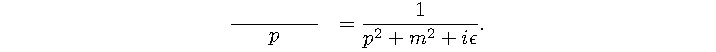
\includegraphics{img/propagator/propagator.pdf}
    \end{center}
    \item Vertex:
    \begin{center}
        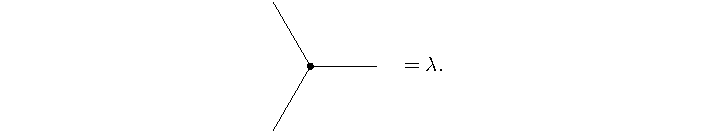
\includegraphics{img/vertex/vertex.pdf}
    \end{center}
\end{itemize}

\plabel{(b)}%
The diagrams are given below.
\begin{center}
    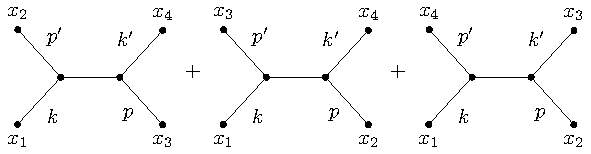
\includegraphics{img/second-order/second-order-2.pdf}
\end{center}
The correlation function is given by
\begin{align*}
    \langle \phi(x_1) \phi(x_2) \phi(x_3) \phi(x_4) \rangle &= \int \dd[d]{y} \int \dd[d]{z} \Delta(x_1 - y)\Delta(x_2 - y)\Delta(x_3 - z)\Delta(x_4 - z) \\
    &\phantom{{}={}} + (x_1,x_2,x_3,x_4 \rightarrow x_1,x_3,x_2,x_4) \\
    &\phantom{{}={}} + (x_1,x_2,x_3,x_4 \rightarrow x_1,x_4,x_2,x_3).
\end{align*}
where
\[ \Delta(r) = \int \frac{\dd[d]{p}}{(2\pi)^d} \frac{e^{ip\cdot r}}{p^2 + m^2 + i\epsilon}. \]

\plabel{(c)}%
The diagrams should satisfy that
\begin{itemize}
    \item $V - E + L = 1$ where $V$ is the number of vertices, $E$ is the number of edges, and $L$ is the number of loops, i.e. $E - L = 7$; and
    \item $2E = \sum_{v} d_v$ where $d_v$ denotes the degree of vertex $v$ and the summation goes through all vertices, i.e. $2E = 4 + 3\times 4$, or $E=8$.
\end{itemize}
Therefore, the diagrams should have $8$ edges and $1$ loop.
Below is the connected diagram of order $\lambda^4$.
\begin{center}
    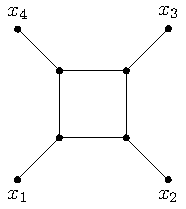
\includegraphics{img/fourth-order/fourth-order.pdf}
\end{center}

\prule

\plabel{4(a)}%
With Wick rotation we find
\begin{align*}
    Z &= \tr[e^{-\beta H}] = \int_{q(\beta) = q(0)} \mathcal{D}q \mathcal{D}p \exp[\int_0^\beta \dd{\tau} \qty(\sum_i p^i \dot{q}^i - H(q,p))] \\
    &= \int_{q(\beta) = q(0)} \mathcal{D}q \exp[-\int_0^\beta \dd{\tau} L_E].
\end{align*}

\plabel{(b)}%
Since
\[ \int \dd{\tau} L_E = \frac{1}{2} \sum_{n\in\mathbb{Z}} \qty[\qty(\frac{2\pi n}{\beta})^2 + \omega^2] \abs{x_n}^2, \]
up to a constant factor we have
\begin{align*}
    Z &= \int \dd{x_0} \prod_{n>0} \int \dd{\Re x_n} \dd{\Im x_n} \exp{-\frac{1}{2} \sum_{n\in\mathbb{Z}}\qty[\qty(\frac{2\pi n}{\beta})^2 + \omega^2] \abs{x_n}^2} \\
    &= \frac{C'}{\omega} \prod_{n>0} \qty[\frac{4\pi^2 n^2}{\beta^2} + \omega^2]^{-1} = \frac{C''}{\beta\omega/2} \prod_{n>0} \qty[1 + \frac{(\beta\omega/2)^2}{(\pi n)^2}] \\
    &= C'' \cdot \frac{1}{\sinh(\beta\omega/2)}.
\end{align*}

\plabel{(c)}%
The Lagrangian is given by
\[ \int \dd{\tau} L_E = \int \dd{\tau} \int \dd[3]{x} \qty[\frac{1}{2} (\partial \phi)^2 + \frac{1}{2} m^2 \phi^2] = \int \dd{\tau} \int \dd[3]{x} \qty[-\frac{1}{2} \phi \partial^2 \phi + \frac{1}{2} m^2 \phi^2]. \]
Applying the Gaussian integral
\begin{gather*}
    \int \mathcal{D}\varphi\, \exp[-\frac{1}{2}\int \dd{^d x} \varphi(x) A\varphi(x) + i \int \dd{^d x} J(x)\varphi(x)] \\
    = \frac{(2\pi)^{(\dim A)/2}}{\sqrt{\det A}} \exp{-\frac{1}{2}\int \dd{^d x} J(x) A^{-1}J(x)}
\end{gather*}
to (for $J=0$)
\[ Z = \int_{\phi(\beta) = \phi(0)} \mathcal{D}\phi \exp[-\int_0^\beta \dd{\tau} L_E] \]
we find (up to a constant factor)
\[ Z = \frac{1}{\sqrt{\det(-\partial^2 + m^2)}}. \]

\plabel{(d)}%
With the expansion
\[ \psi(\tau) = \beta^{-1/2} \sum_{n\in \mathbb{Z}} e^{(2n+1)\pi i\tau/\beta} \psi_n \]
we find
\begin{align*}
    Z &= C\int \prod_n \dd{\overline{\psi}_n}\dd{\psi_n} \exp[- \sum_n \overline{\psi}_n \qty(\frac{(2n+1)\pi i}{\beta} + \omega) \psi_n] \\
    &= C \prod_{n} \qty(\frac{(2n+1)\pi i}{\beta} + \omega) \\
    &= C \prod_{n\ge 0} \qty(\omega^2 + \frac{(2n+1)^2 \pi^2}{\beta^2}) \\
    &= C' \cosh(\frac{\beta\omega}{2}).
\end{align*}

\end{document}
